%% ============================================================================
%%
%%  Master's thesis
%% 
%%  Author: FORNAVN EFTERNAVN
%%
%%  Chapter 1: Coffee
%% ============================================================================

\chapter{BBN physics and cosmology}
\label{chap:theory}

To understand the process of Big Bang nucleosynthesis, we must examine the intersection between Cosmology, thermodynamics, particle, and nuclear physics. Though this might seem daunting, it turns out that the unique conditions during this epoch allow for extensive simplifications of this otherwise monumental task. Throughout this section we use $\hbar=c=k_B=1$.



% ~~~~~~~~~~~~~~~~~~~~~~~~~~~~~~~~~~~~~~~~~~~~~~~~~~~~~~~~~~~~~~~~~~~~~~~~~~~~~
% SECTION
% ~~~~~~~~~~~~~~~~~~~~~~~~~~~~~~~~~~~~~~~~~~~~~~~~~~~~~~~~~~~~~~~~~~~~~~~~~~~~~
\section{Determining background parameters}
\label{sec:Background}

\subsection{Temperature and scale factor}
\label{ssec:cosmology}

BBN takes place after inflation while the universe is still radiation dominated. This can be described by the Friedman equation, which can be further simplified with the reasonable approximation, that both curvature and the cosmological constant are zero. 
\begin{align}
    H^2=\left(\frac{\dot{a}}{a}\right)^2=\frac{8\pi G}{3}\rho_{tot}
\end{align}
With $\rho_{tot}$ referring to the total energy density of photons, leptons and baryons.
\begin{align}
    \rho_{tot}=\rho_{\gamma}+\rho_{\nu}+(\rho_{e^-}+\rho_{e^+})+\rho_{b}
\end{align}
This equation can be rewritten as the differential equation explicitly describing the time evolution of the scale factor.
\begin{align}
    \diff{a}{t}=a\sqrt{\frac{8\pi G}{3}\rho_{tot}(T,a)}
    \label{eq:dadt}
\end{align}
To find an expression for the temperature evolution, we use energy conservation. We can consider the neutrinos as decoupled during BBN, and so the photon temperature will be determined by the remaining components. Since this point the universe is very much homogeneous and isotropic, we utilize the fluid equation for adiabatic expansion \cite[{(4.44)}]{Ryden}. 
\begin{align}
    \dot{\rho_{set}}+3\frac{\dot{a}}{a}(\rho_{set} + P_{set})=0
\end{align}
With $\rho_{set}$ being the density of none-decoupled components and $P_{set}$ being their pressures.
\begin{align}
    \rho_{set}=\rho_{\gamma}+(\rho_{e^-}+\rho_{e^+})+\rho_{b}
    \eqsep P_{set}=P_{\gamma}+(P_{e^-}+P_{e^+})+P_{b}
\end{align}

Using the chain rule we can then set up a differential equation describing the time evolution of the photon temperature. 
\begin{align}
    \diff{T}{t}=-3\frac{\dot{a}}{a}\frac{\rho_{set}(T,a) + P_{set}(T,a)}{\diff{\rho_{set}(T,a)}{T}}
    \label{eq:dTdt}
\end{align}

\subsection{Additional parameters}
Most BBN codes are based on the original code by Wagoner described in section \ref{sec:BBN_history}. These don't track the scale factor, but instead use the quantity $h$.
\begin{align}
    h=M_u\frac{n_{b}}{T^3_9}
\end{align}
$M_u$ being atomic mass units, $n_b$ the baryon number density, and  $T_9$ the temperature in $10^9$ Kelvin. This quantity was useful since it stays approximately constant throughout BBN, while being easy to directly convert to baryon density. However, with modern computers this numerical simplicity is inconsequential, and as such it is more reasonable to track the scale factor.
The electron chemical potential was also tracked by the Wagoner code and its successors. The only effect of this is ensuring a non-zero electron density after reheating. We can easily set this to 0, as the impact will be 3 orders of magnitude lower than the already miniscule impact of the baryon density.

\textcolor{orange}{Neutrino temperature?}


\section{Energy densities and pressure}

In the very early universe most particles were in thermal equilibrium, and can be described by the rules of statistical physics. The average number of particles in a given state is governed by the Fermi-Dirac distribution for fermions, and the Bose-Einstein distribution for bosons.
\begin{align}
    \bar{n}_{FD}=\frac{1}{e^{(E-\mu)/T}+1} \eqsep   \bar{n}_{BE}=\frac{1}{e^{(E-\mu)/T}-1}
    \label[equation]{fermionboson}
\end{align}
With $E$ being the total energy each particle in the state and $\mu$ the chemical potential. The number density can be found generally by integrating over all possible momentum states. 
\begin{align}
    n(T)=\frac{g}{(2\pi)^3}\int_{0}^{\infty}\bar{n}(p,T)dp^3=\frac{g}{2\pi^2}\int_{0}^{\infty}\bar{n}(p,T) p^2 dp
    \label[equation]{numberdensity}
\end{align}
With g being the degeneracy parameter. We can similarly find an expression for the energy density by multiplying the integrand by the relativistic energy $E^2=m^2+p^2$.
\begin{align}
    \rho(T)=\frac{g}{2\pi^2}\int_{0}^{\infty}\bar{n}(p,T)\sqrt{m^2+p^2} p^2 dp
    \label[equation]{energydensity}
\end{align}
Pressure is defined as the force exerted per unit area. Consider a relativistic particle confined to a sphere of radius $r$. Whenever it collides with the surface, it will exert a force proportional to the change in momentum. 
\begin{align}
    F=\diff{p}{t}=\frac{\Delta p }{\Delta t}\eqsep
    \Delta p = 2p \cos \theta
\end{align}
With $\theta$ being the incident angle. 

The time between collisions can be deduced based on the distance traveled. 
\begin{align}
    \Delta t = \frac{L}{\mathrm{v}}=L\frac{\sqrt{m^2+p^2}}{p}
\end{align}
With distance between collisions $L$ and velocity $\mathrm{v}$.

Next, consider the triangle created by the center of the sphere and two consecutive collision points. Using the law of cosines we can determine $L$.
\begin{align}
    r^2=L^2+r^2+2L r \cos \theta \Rightarrow
    L = 2r \cos \theta
\end{align}
We can then determine the force and pressure exerted on the sphere by each particle. 
\begin{align}
    F = \frac{p^2}{r\sqrt{m^2+p^2}} \eqsep P = \frac{p^2}{4\pi r^3\sqrt{m^2+p^2}}
\end{align}
Generalizing this for any volume, we get the integral for the total pressure of a relativistic gas.
\begin{align}
    PV=\frac{p^2}{3\sqrt{m^2+p^2}} 
    \label[equation]{Pcontribution}
\end{align}
\begin{align}
    P(T)=\frac{g}{6\pi^2}\int_{0}^{\infty}\bar{n}(p,T)\frac{p^4}{\sqrt{m^2+p^2}}dp
    \label[equation]{pressure}
\end{align}
Additionally, we see that the pressure of an ultra-relativistic gas follows a simple relation.
\begin{align}
    P(T)=\frac{\rho(T)}{3} \quad (\text{for } m\ll p)
    \label[equation]{Prho3}
\end{align}

\subsection{Photons}


Photons are massless bosons with 2 distinct polarizations, for each momentum state. With $g=2$, we use \ref{energydensity} to determine the energy density. 
\begin{align}
    \rho_\gamma(T)=\int_{0}^{\infty} \frac{p^3}{\pi^2}\frac{1}{e^{p/T}-1}dp =  \frac{T^4}{\pi^2}\int_{0}^{\infty}\frac{u^3}{e^{u}-1}du
\end{align}
This integral is a well know representation of the Riemann Zeta function \cite[\href{https://dlmf.nist.gov/25.5.E1}{(25.5.1)}]{NIST:DLMF}.
\begin{align}
    \rho_\gamma(T)=\frac{T^4}{\pi^2}\Gamma(4)\zeta(4)=\frac{\pi^2}{15}T^4
    \label[equation]{rhogamma}
\end{align}
Now we can easily define the temperature derivative and pressure.
\begin{align}
    \diff{\rho_\gamma(T)}{T}=\frac{4}{15}\pi^2T^3 \eqsep P_\gamma(T)=\frac{\rho_\gamma(T)}{3}
\end{align}




\subsection{Neutrinos}

For neutrinos $g=2N_\nu$, to account for the different species and their antiparticles.
\begin{align}
    \rho_\nu(T_\nu)=N_\nu\int_{0}^{\infty} \frac{p^3}{\pi^2}\frac{1}{e^{p/T_\nu}+1}dp =  N_\nu\frac{T_\nu^4}{\pi^2}\int_{0}^{\infty}\frac{u^3}{e^{u}+1}du
\end{align}
This is also an integral representation of the Riemann Zeta function \cite[\href{https://dlmf.nist.gov/25.5.E3}{(25.5.3)}]{NIST:DLMF}.
\begin{align}
    \rho_\nu(T_\nu)=N_\nu\frac{T_\nu^4}{\pi^2}\Gamma(4)\zeta(4)(1-2^3)=N_\nu\frac{7}{8}\frac{\pi^2}{15}T_\nu^4
    \label[equation]{rhonu}
\end{align}
The effective neutrino number is $N_\nu=3.046$ to take into account various QFT corrections\cite{Mangano_2005}.

Tracking the neutrino temperature separately is quite troublesome, luckily we don't have to. Since neutrinos decouple very early, the only significant change in their energy density will be due to the expansion of the universe. Therefore, we can track the later evolution using the scale factor.
\begin{align}
    \rho_\nu(t)=\frac{\rho_\nu(T_i)}{a(t)^4}
    \label[equation]{realrhonu}
\end{align}



\subsection{Electrons and positrons}


Electrons and positrons unfortunately have mass, which makes solving for their density and pressure much more troublesome.
\begin{align}
    \rho_\pm(T)=\frac{1}{\pi^2}\int_{0}^{\infty}\frac{\sqrt{m^2+p^2}}{e^{(E\pm\mu)/T}+1}p^2 dp
    \label[equation]{rhoe}
\end{align}
\begin{align}
    P_\pm(T)=\frac{1}{3\pi^2}\int_{0}^{\infty}\frac{1}{e^{(E\pm\mu)/T}+1}\frac{p^4}{\sqrt{m^2+p^2}} dp
\end{align}
Inspired by the derivation of Chandrasekhar \cite{Chandrasekhar}, we will solve these integrals by using the rapidity $\theta$.
\begin{align}
    \sinh \theta = \frac{p}{m}\eqsep \cosh \theta = \frac{E}{m}
    \label[equation]{rapiditet}
\end{align}
After a simple change of variable we get a much nicer form of the integrals.
\begin{align}
    \rho_\pm(T)=\frac{m^4}{\pi^2}\int_{0}^{\infty}\frac{\sinh^2 \theta \cosh^2\theta}{e^{(m \cosh\theta\pm\mu)/T}+1} d\theta
    \label[equation]{rhoet}
\end{align}
\begin{align}
    P_\pm(T)=\frac{m^4}{3\pi^2}\int_{0}^{\infty}\frac{\sinh^4 \theta}{e^{(m \cosh\theta\pm\mu)/T}+1} d\theta
    \label[equation]{Pet}
\end{align}
Before and during BBN $(E\pm\mu)/T $ will be strictly positive, and we can therefore perform a series expansion, which converges nicely for high temperatures.
\begin{align}
    \frac{1}{e^{(m \cosh\theta\pm\mu)/T}+1}=\sum_{n=1}^{n=\infty} (-1)^{n+1} e^{-n\frac{m }{T}\cosh\theta}e^{\mp n\frac{\mu}{T}}
\end{align}
The chemical potential does not depend on the rapidity, allowing us to get combined pressure of both electrons and positrons.
\begin{align}
    P_e(T)=P_-+P_+=\frac{2m^4}{3\pi^2}\sum_{n=1}^{n=\infty} (-1)^{n+1} \cosh{\left(n\frac{\mu}{T}\right)}  \int_{0}^{\infty}e^{-n\frac{m }{T}\cosh\theta}\sinh^4 \theta d\theta
\end{align}
These terms are integral representations of modified Bessel functions \cite[\href{https://dlmf.nist.gov/10.32.E8}{(10.32.8)}]{NIST:DLMF}.
\begin{align}
    \int_{0}^{\infty}e^{-z\cosh\theta}\sinh^4 \theta d\theta=4\frac{\Gamma(2+\frac{1}{2})}{\sqrt{\pi}z^2}K_2\left(z\right)=3z^{-2}K_2\left(z\right)
\end{align}
With $z=n\frac{m }{T}$, we can get the total pressure expressed as a sum of modified Bessel functions.
\begin{align}
    P_e(T)=\frac{2m^2}{\pi^2} T^2 \sum_{n=1}^{n=\infty} \frac{(-1)^{n+1}}{n^{2}} \cosh{\left(n\frac{\mu}{T}\right)}   K_2\left(n\frac{m }{T}\right)
    \label{Pelectron}
\end{align}
The energy density can be found by the same way, by first utilizing the identity $cosh^2=sinh^2+1$, to get the energy density in terms of $\sinh\theta$.
\begin{align}
    \rho_e(T)=\rho_-+\rho_+=\frac{2m^4}{\pi^2}\sum_{n=1}^{n=\infty} (-1)^{n+1} \cosh{\left(n\frac{\mu}{T}\right)}  \int_{0}^{\infty}e^{-n\frac{m }{T}\cosh\theta}\left(\sinh^4\theta +\sinh^2\theta\right) d\theta
\end{align}
The $\sinh^4$ term is clearly the same as for the pressure up to a factor of 3. Comparing this to the results for massless particles, this term can be interpreted as the relativistic pressure of the electron gas. The second term also corresponds to a modified Bessel function, though of first rather than second order \cite[\href{https://dlmf.nist.gov/10.32.E8}{(10.32.8)}]{NIST:DLMF}. Combined this grants us the sum describing the total energy density of electrons and positrons.
\begin{align}
    \rho_e(T)=\frac{2m^2}{\pi^2} T^2 \sum_{n=1}^{n=\infty} \frac{(-1)^{n+1}}{n^{2}} \cosh{\left(n\frac{\mu}{T}\right)}  \left( 3 K_2\left(n\frac{m }{T}\right) + n\frac{m }{T} K_1\left(n\frac{m }{T}\right) \right)
    \label{rhoelectron}
\end{align}
Using recursion relations for the modified Bessel functions \cite[\href{https://dlmf.nist.gov/10.29.E1}{(10.29.1)}]{NIST:DLMF}, we see that this is equivalent to the expression used in other BBN codes \cite{Kawano}.
\begin{align}
3K_{2}(z)+z K_{1}(z)=3\frac{z}{4}[K_{3}(z)-K_{1}(z)]+z K_{1}(z)=\frac{z}{4}[3K_{3}(z)+K_{1}(z)]
\end{align}
\begin{align}
    \rho_e(T)=\frac{m^3}{2\pi^2} T \sum_{n=1}^{n=\infty} \frac{(-1)^{n+1}}{n} \cosh{\left(n\frac{\mu}{T}\right)}  \left( 3 K_3\left(n\frac{m }{T}\right) + K_1\left(n\frac{m }{T}\right) \right)
\end{align}
As mentioned many older BBN codes track the parameter $\phi_e=\frac{\mu}{T}$, but this is unnecessary, as the electron density after reheating is 3 orders of magnitude lower than the already negligible contribution of the baryons. So for the remaining calculation we set $\mu = 0$.

Finding the temperature derivative of the electron energy density, can also be achieved using the recursion relations for Bessel functions \cite[\href{https://dlmf.nist.gov/10.29.E2}{(10.29.2)}]{NIST:DLMF}.
\begin{align}
    \diff{}{z} \frac{1}{z}[3K_{3}(z)+K_{1}(z)]&=-3[z^{-2} K_{3}(z)+z^{-1} K_{2}(z)+ 3z^{-2} K_{3}(z)]-z^{-1} K_{2}\\
    &=-12 z^{-2} K_{3}(z)-4z^{-1} K_{2}(z)\\
    &=-\frac{1}{z}[2K_{4}(z)-2K_{2}(z)+4 K_{2}(z)]\\
    &=-\frac{2}{z}[K_{4}(z)+K_{2}(z)]
\end{align}
Multiplying by $\idiff{z}{T}$ we get the complete derivative.
\begin{align}
    \diff{\rho_e(T)}{T}=\frac{m^4}{\pi^2} \frac{1}{T} \sum_{n=1}^{n=\infty} (-1)^{n+1}   \left(K_4\left(n\frac{m }{T}\right) + K_2\left(n\frac{m }{T}\right) \right)
\end{align}


\subsection{Baryons}





The temperatures at which BBN takes place are too low for Baryon pair production. Therefore, the number density of baryons can be solely determined by the scale factor and some known density. 
\begin{align}
    n_b(a)=\frac{a_0^3}{a^3}n_{b}(a_0)
\end{align}
To determine baryon density $n_{b}(a_0)$, we use the baryon photon/ratio $\eta$. 
\begin{align}
    n_b=n_\gamma(T) \eta \eqsep n_\gamma(T)=\frac{T^3}{\pi^2}\Gamma(3)\zeta(3)
\end{align}
From the CMB we can measure the value of $\eta$, during recombination, but unlike baryons the number of photons does not remain unchanged from the start of BBN until recombination. The only significant source of photons is the annihilation of the electron-positron pairs. We can account for this using conservation of entropy. For a given species we define the entropy density \cite[(3.91)]{kolbturner}.
\begin{align}
    s=\frac{\rho+P}{T}
\end{align}
Setting $a=1$ at the start of our BBN calculations, we get a relation between the total entropy before and after annihilation.
\begin{align}
     s_{\gamma}(T_{CMB})a_{CMB}^3= s_e(T_{i})+s_{\gamma}(T_{i})
    \label{eq:entropycon}
\end{align}
The photon number density is directly proportional to entropy density, both scaling with $T^3$. This allows us to restate \ref{eq:entropycon} only in terms of the initial entropy density.
\begin{align}
    n_{\gamma}(T_{CMB})a_{CMB}^3 = \frac{n_\gamma(T_{i})}{s_{\gamma}(T_{i})}\left(s_e(T_{i})+s_{\gamma}(T_{i})\right)
\end{align}
From this we get the baryon density as a function of the initial photon and electron density and pressure.
\begin{align}
    n_b(a_{CMB}){a_{CMB}^3}=n_\gamma(T_{i}) \left(\frac{s_e(T_{i})+s_{\gamma}(T_{i})}{s_{\gamma}(T_{i})}\right)\eta
\end{align}
\begin{align}
    n_b(a)=\frac{1}{a^3}n_\gamma(T_{i}) \left(1+\frac{\rho_e(T_{i})+P_{e}(T_{i})}{\rho_{\gamma}(T_{i})+P_{\gamma}(T_{i})}\right)\eta
\end{align}
With $T_i$ being the initial temperature. Finally, to get the energy density we simply need to sum over all different nuclei. 
\begin{align}
    \rho_b(a)=n_b(a)\sum_{i}^{}Y_i m_i
    \label{rhob}
\end{align}
For each isotope $m_i$ is the mass, and $Y_i$ is the ratio between the number of nuclei and the total number of nucleons. $Y_i$ is often defined as $Y_i=X_i/A_i$, with $X_i$ being the mass fraction, and $A_i$ the atomic weight \cite{Wagoner69}. The difference in per nucleon mass of different isotopes, causes these two definitions to have a relative difference of \num{1e-5}, which can be safely neglected. Furthermore, since eta is only known with an accuracy of $1\%$ \cite{Planck}, we can approximate that all baryons have the same mass as a lone proton reducing \ref{rhob} to $\rho_b(a) \approx n_b(a)m_p$.

The baryon pressure can be found using the ideal gas law.
\begin{align}
    P_b(a)= n_b(a)T\sum_{i}^{}Y_i
\end{align}
Unlike for the relativistic particles, the baryon pressure is several orders of magnitude lower than the density. Since the baryon density is already comparatively low, the pressure will be completely negligible.
%invm=A**2/m_Nucs
%def altrho_bY_cgs(y):
%return eta_ini*n_gamma_ini/y[1]**3*gcm3/np.dot(y[n_bparams:6+n_bparams],invm[:6])
%plt.figure()
%plt.plot(soltime/timeunit,np.array([a_cache(soltime[i])**3*rho_bY_cgs(np.array([T_cache(soltime[i]),a_cache(soltime[i])]+list(solY[:,i]))) for i in range(len(soltime))])/np.array([a_cache(soltime[i])**3*altrho_bY_cgs(np.array([T_cache(soltime[i]),a_cache(soltime[i])]+list(solY[:,i]))) for i in range(len(soltime))]),label='Normal density')

%
%
% ~~~~~~~~~~
% SUBSECTION
% ~~~~~~~~~~
\section{Nuclear reactions}
\label{sec:nucleartheory}

All relevant nuclear reactions involve at most 6 different nuclei. Generally we can write these reactions as
\begin{align}
    N_i X_i + N_j X_j + N_k X_k \leftrightharpoons N_n X_n + N_m X_m + N_l X_l ,
\end{align}
where $N_i$ is the number of nuclei $X_i$, that enter the reaction. 
The change in abundance $Y_i$ of any nuclei is given by the sum of all reactions that create or destroy it.
\begin{align}
    \diff{Y_i}{t}=\sum_\lambda\frac{N_i}{n_b}\left(\lambda_{n m l \rightarrow i j k} \frac{Y_n^{N_n}Y_m^{N_m}Y_l^{N_l}}{N_n!N_m!N_l!}n_b^{(N_n+N_m+N_l)}-\lambda_{i j k \rightarrow n m l}\frac{Y_i^{N_i}Y_j^{N_j}Y_l^{N_k}}{N_i!N_j!N_k!}n_b^{(N_i+N_j+N_k)}\right)
    \label{dYdt}
\end{align}
With $\lambda$ being the reaction rate, and $n_b$ the baryon number density. 

\subsection{Proton $\leftrightharpoons$ neutron rate}
This section should probably be in the BBN code chapter



%\chapter{Nuclear abundances}

\section{Initial conditions}

\subsection{Initial temperature}
When performing BBN calculations, it is most sensible to choose an initial temperature, and from it, determine all other initial conditions. The chosen temperature should be sufficiently high, so that all particles are in thermal equilibrium. Most BBN codes use \num{2.7e10} K as the initial temperature. Higher temperatures could be used, but this is unnecessary and will often lead to numerical instabilities, which I will touch upon in Chapter \ref{chap:BBNcode}.

\subsection{Initial time}

Though none of the equations describing BBN, have any explicit time dependence, it is still nice to know the age of the universe when it takes place. This can be achieved by integrating equation \eqref{eq:dTdt}, with $T=\infty$ at $t=0$.
\begin{align}
    %\diff{T}{t}=\mp\sqrt{24\pi G\rho_{tot}}\frac{\rho_{set}(T,a) + P_{set}(T,a)}{\diff{\rho_{set}(T,a)}{T}}\\
    \int_{0}^{t_i}dt=-\int_{\infty}^{T_i}(24\pi G\rho_{tot})^{-1/2}\frac{\diff{\rho_{set}(T)}{T}}{\rho_{set}(T) + P_{set}(T)}dT
\end{align}
For high temperatures we can assume that the electrons are completely relativistic. Based on the result for neutrinos \eqref{rhonu}, we know that the energy of a massless fermion differs from that of a boson by a factor of $7/8$. Accounting for the g factors, we get $\rho_e=7/4 \rho_\gamma$. At temperatures above 2 MeV the relativistic approximation deviates by less than 1\%, see figure \ref{fig:rhoegammaT}.
\begin{figure}[h!]
    %\centering
    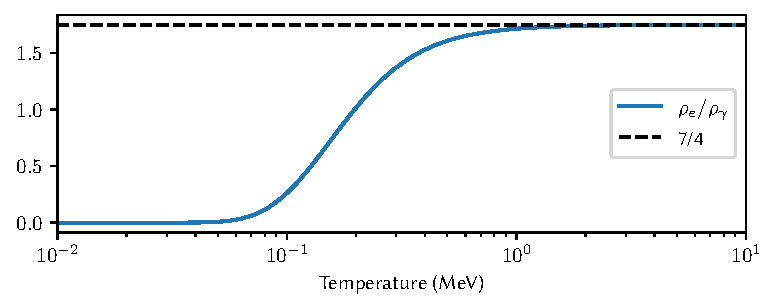
\includegraphics[width=5.1in]{figures/rhoegammaT.pdf}
    \caption{Exact ratio of the electron-positron energy to the photon energy}
    \label{fig:rhoegammaT}
\end{figure}

At these temperatures we can safely ignore the baryon contribution, which combined with \eqref{Prho3}, allows us to calculate the non-decoupled terms.
\begin{align}
    \frac{\diff{\rho_{set}(T)}{T}}{\rho_{set}(T) + P_{set}(T)}=\frac{3}{4}\frac{1}{\rho_{set}(T)}\diff{\rho_{set}(T)}{T}=3T^{-1}
\end{align}
For the total energy we simply add the contributions of all components, excluding baryons,
\begin{align}
    \rho_{tot}=\rho_\gamma+(2+N_\nu)\frac{7}{8}\rho_\gamma=\frac{43}{8}\rho_\gamma
\end{align}

\begin{align}
    t_i&=3(24\pi G\frac{43}{8}\frac{\pi^2}{15})^{-1/2}\int_{\infty}^{T_i}T^{-3}dT\\
    t_i&=\frac{3}{2}( \frac{43}{5}G\pi^3)^{-1/2}T_i^{-2}
    \label{eq:t_ini}
\end{align}
In units of \num{1e9} K, and seconds This can be written as,
\begin{align}
    T_9=( 43 \frac{4}{3}\pi\frac{a}{c^2}G)^{-1/4}t^{-1/2}=9.97t^{-1/2},
\end{align}
with $a$ being the radiation constant, related to the Stefan–Boltzmann constant by $a=\frac{4}{c}\sigma$. This differs significantly from the expression derived by Wagoner\cite{Wagoner67},
\begin{align}
    T_9=(12\pi\frac{a}{c^2}G)^{1/4}t^{-1/2}=10.4t^{-1/2},
\end{align}
The analytical expression is wrong, but the numerical result is correct. A simple error which probably was the result of a small mistake when transcribing the notes used for the paper. This expression has been reproduced in several later BBN codes such as Kawano\cite{Kawano} and ALterBBN\cite{AlterBBN}. Though Kawano reproduced the equation in the documentation, in the actual NUC123 code, he used the numerical result and as such the code itself had no errors. In AlterBBN they used natural units, and therefore couldn't use the numerical value, and therefore the error affected their result. Additionally, they also confused the Stefan–Boltzmann and radiation constants leading to an additional error. Examining the code, one can see that their value is wrong by 14 orders of magnitude. %which they seemly discovered and erroneously corrected by doing an additional conversion from $\hbar/GeV$ to seconds. This brings the final value to a few mi
Since it doesn't impact final abundances, this error was only very recently discovered. The first correction being released in 2021 by Sharpe \cite{sharpe2021big},
\begin{align}
    T_9=(48\pi\frac{a_r}{c^2}G)^{-1/4}t^{-1/2}=10.4t^{-1/2},
\end{align}
However this still differs from \eqref{eq:t_ini}. This due to the fact that the original derivation was performed by Wagoner in 1967, a decade before the discovery of the Tau and corresponding neutrino. And though everyone correctly added the additional neutrino flavor when calculating the neutrino energy, it seems everyone forgot to consider the impact it has on the initial time. 

Using \eqref{eq:t_ini} we can also justify the omission of particles heavier than electrons. The lightest of these are the muon and pion, which both have masses above 100 MeV. As such they will only start contributing at time less than a millisecond. 

%Warning test\fxwarning{This is a warning!}


\section{solving things}
